% xetex compatible variant that support TTF fonts according to company rules
\documentclass[ignorenonframetext, professionalfonts, hyperref={unicode}]{beamer}

\usetheme{Epam}

\usepackage{fontspec}
\setsansfont{SourceSansPro-Regular}
%\setbeamerfont{frametitle}{family=\fontspec{Oswald}}
\setbeamerfont{frametitle}{family=\fontspec{Oswald}}
\setbeamerfont{block title}{family=\fontspec{Oswald}}

%\setmainfont{Times New Roman}
\defaultfontfeatures{Mapping=tex-text}
\defaultfontfeatures{Ligatures=TeX}

%\setsansfont{Arial}
%\setromanfont{Trebuchet MS}

\usepackage{cmap}
\usepackage{graphicx}

\usepackage{textcomp}

\usepackage{beamerthemesplit}

\usepackage{ulem}

\usepackage{verbatim}
\usepackage{import}

\usepackage{listings}
\lstloadlanguages{bash}

\lstset{escapechar=`,
	captionpos=b,
	extendedchars=false,
	language=sh,
%	frame=single,
	tabsize=2, 
	columns=fullflexible, 
%	basicstyle=\scriptsize,
	keywordstyle=\color{blue}, 
	commentstyle=\itshape\color{brown},
%	identifierstyle=\ttfamily, 
	stringstyle=\mdseries\color{green}, 
	showstringspaces=false, 
	numbers=left, 
	numberstyle=\footnotesize, 
	breaklines=true, 
	inputencoding=utf8,
	keepspaces=true,
	morekeywords={u\_short, u\_char, u\_long, in\_addr}
	}

\definecolor{darkgreen}{cmyk}{0.7, 0, 1, 0.5}

\lstdefinelanguage{diff}
{
    morekeywords={+, -},
    sensitive=false,
    morecomment=[l]{//},
    morecomment=[s]{/*}{*/},
    morecomment=[l][\color{darkgreen}]{+},
    morecomment=[l][\color{red}]{-},
    morestring=[b]",
}

\author[Epam]{{\bf Epam}\\Low Level Programming Department}

%\institution[EPAM]{EPAM}
%\logo{\includegraphics[width=1cm]{logo.png}}

\graphicspath{{../../slides/cmdline/clipart/}{../../slides/bash/clipart/}}

\bibliographystyle{unsrt}
\setbeamertemplate{bibliography item}{\insertbiblabel}

\AtBeginSection[]{%
  \begin{frame}<beamer>
    \frametitle{}
    \tableofcontents[
        sectionstyle=show/shaded, hideallsubsections ]
  \end{frame}
  \addtocounter{framenumber}{-1}% If you don't want them to affect the slide number
}

% \regex for regular expressions
\newcommand{\regex}[1]{ %
\expandafter{$\ulcorner{\color{blue}\texttt{#1}}\lrcorner$} %
}



\title{Введение в GNU/Linux}

%%%%%%%%%%%%%%%%%%%%%%%%%%%%%%%%%%%%%%%%%%%%%%%%%
%%%%%%%%%% Begin Document  %%%%%%%%%%%%%%%%%%%%%%
%%%%%%%%%%%%%%%%%%%%%%%%%%%%%%%%%%%%%%%%%%%%%%%%%

\begin{document}

\begin{frame}
	\frametitle{}
	\titlepage
	\vspace{-0.5cm}
	\begin{center}
	%\frontpagelogo
	\end{center}
\end{frame}


\begin{frame}
	\tableofcontents
	[hideallsubsections]
\end{frame}

%%%%%%%%%%%%%%%%%%%%%%%%%%%%%%%%%%%%%%%%%   
%%%%%%%%%% Content starts here %%%%%%%%%%
%%%%%%%%%%%%%%%%%%%%%%%%%%%%%%%%%%%%%%%%%

\section{О курсе}

% add one slide with unix/linux history, age, culture, motivation why it is important to learn
% \mode<all>{\begin{frame}{About myself.}

    \large Vikentsi Lapa - Senior Software Test Automation Engineer
    \begin{columns}
        \column{0.6\textwidth}
            \begin{itemize}
                \item Hands on experience with Linux about 8 years in such areas as
                \begin{itemize}
                    \item High Perfomance Computing
                    \item Cluster file systems: GPFS, Lustre 
                \end{itemize}
                \item MLUG (Minsk Linux User Group Activist) and LVEE conference participant 
            \end{itemize}
        \column{0.3\textwidth}
            \center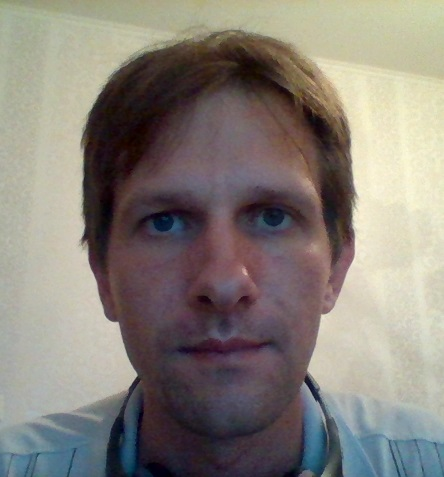
\includegraphics[width=3cm]{myphoto}
    \end{columns}
\end{frame}

\begin{frame}{Cложность изучения системы.}
         \center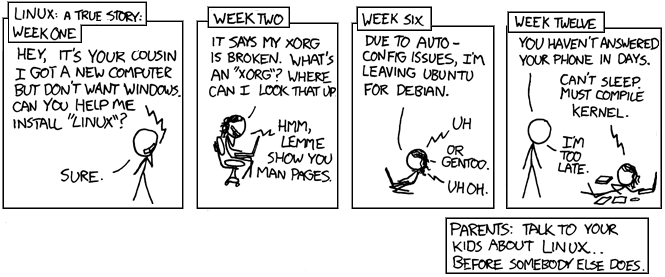
\includegraphics[scale=0.6]{linux_story} 
    \break
\pause
Сложности: множество вариантов, обилие информации, терминология, новые интерфейсы, ошибки.
\pause
	\begin{center}
		\large
		Обеспечить быстрый старт в среде GNU/Linux для опытных пользователей. Понизить порог вхождения. Задать направление. 
	\end{center} 
\end{frame}


\begin{frame}{Аудитория}

Кому полезен этот курс:
\begin{itemize}
    \item IT Engineers, DevOps Engineers
    \item Junior Software Engineers/Software Engineers
    \item Test Engineers, Test Automation Engineers
    \item Students
\end{itemize}
    \pause
Что требуется от вас:
\begin{itemize}
    \item Опыт работы с Linux/Unix меньше 1 года или без опыта
    \pause
    \item Опыт работы с системой виртуализации
    \item Знание сетевых технологий
    \item Creative thinking and problem solving skills
    \pause
    \item \alert{Feedback is essential: answer to questions, do practical tasks, do homework, ask questions}
\end{itemize}
\end{frame}

\begin{frame}{Проверим обратную связь}
\begin{itemize}
    % this one moved to email trainee introduction
    %\item Есть ли опыт работы с Linux? Если есть то сколько?
    %\pause
    %\item Ваши ожидания. Зачем пришли на курс?
    %\pause
    \item Установили дистрибутив? Какой?
    \item Если не установили напишите причину.
\end{itemize}
\end{frame}

\begin{frame}[fragile]{Оценка возраста системы Unix.}
Ваша версия.
 \pause
\begin{lstlisting}
    $ date --help | grep '%s'
    $ date +%s # show current date in seconds 
    $ echo $(( $(date +%s)/(60*60*24*365))) # show years
\end{lstlisting} 
\pause
Unix systems are characterized by a \alert{modular design} or ``Unix philosophy"
		\begin{columns}
		\column{0.7\textwidth}
\begin{itemize}
    \item simple tools that each perform a limited, well-defined function
    \item shell scripting and command language to combine the tools to perform complex workflows
    \item unified filesystem
\end{itemize}
		\column{0.3\textwidth}
            
\includegraphics[width=4cm]{40years}
		\end{columns}
% За это время сложилась культура и философия разработки, которая оказала влияние на интерфейсы взаимодействия, например названия устройств и команд.
% Разнообразие подходов при решении задач. Среда дружественная для программиста и опытного технического пользователя.
\end{frame}


%\begin{frame}{Состав курса}
%	\begin{itemize}
%		\item Представление об архитектуре GNU/Linux дистрибутива
%			\pause
%		\item "Ежедневные" навыки работы в консоли. Конфигурация системы.
%			\pause
%		\item Язык программирования
%			\begin{itemize}
%					\item shell (Bash)
%			\end{itemize}
%			\pause
%		\item Все, чего вы не знали и боялись спросить
%	\end{itemize}
%\end{frame}
}
\mode<all>{\begin{frame}[fragile]
\frametitle{Синтаксис {\bf if}}

	\begin{columns}
		\column{0.5\textwidth}
	
	\begin{lstlisting}[language=bash]
if command1
then
    OTHER COMMANDS
elif command2
then
    OTHER COMMANDS
else
    OTHER COMMANDS
fi
\end{lstlisting}
		\column{0.5\textwidth}
Варианты форматирования
then отдельной строкой
	\begin{lstlisting}[language=bash]
if command
then OTHER COMMANDS 
fi
\end{lstlisting}

then и if на одной строке
	\begin{lstlisting}[language=bash]
if command; then 
    OTHER COMMANDS
fi
\end{lstlisting}
	\end{columns}

В зависимости от результата выполнения (exit code) command1 выполняется блок команд после then.   

Ключевое слово fi - обязательно

%	\pause
%	{\bf Практическое задание:} \\
%	\begin{itemize}
%
%		\item с помощью конструкции {\bf if} проверить существует ли файловый объект передаваемый в качестве параметра скрипту ({\tt man test})
%		\item если нет, то создать директорию с таким именем
%		\item если cуществует и файл является shell-скриптом ({\tt man file}), то запустить его
%		\item если существует и является директорией, то вывести на экран Top5 по размеру файлов из этой директории, 
%		    отсортированных в порядке убывания ({\tt man ls, man head})
%%	\end{itemize}
%	\end{columns}
\end{frame}
}
\mode<all>{\begin{frame}[fragile]{Владельцы файла. Внутреннее представление}
  \begin{itemize}
    \item \alert{Владелец-пользователь} и \alert{владелец-группа} файла определяются по идентификаторам \alert{UID}\footnote{UID - User IDentifier} и \alert{GID}\footnote{GID - Group IDentifier}, а не по именам. 
\lstinputlisting{../../slides/cmdline/samples/ls-nl} \pause
    \item Зарегистрированные пользователи и группы определены в файлах \alert{/etc/passwd} и \alert{/etc/group} \newline
    Следствие: могут существовать файлы, принадлежащие не зарегистрированным в системе пользователям и группам. \pause
    \item Новые файлы создаются с владельцем-пользователем, запустившим команду создания и его первичной группой, как владельцем группой. \pause
  \end{itemize}

\end{frame}
}
\mode<all>{\begin{frame}
\frametitle{Время знакомиться}
Встали и расположились, так чтобы видеть всех участников тренинга \\
\begin{itemize}
    \item Как зовут? 
    \item Где и как планируете применять знания системы Linux?
\end{itemize}
\end{frame}
}
\mode<all>{\begin{frame}
\frametitle{Время знакомиться}
    Разбились на 2 команды
\begin{itemize}
    \item Каждый вспомнит несколько фактов про системного администратора (Linux)
    \item Например: Веселый, cтереотип, поведение, особенность профессии.
    \item Через 5 мин сравним, что получилось у каждой команды.
\end{itemize}
\end{frame}
}

%\mode<all>{\begin{frame}[fragile]
   \frametitle{Команды сравнения.}

\underline{Выполнить команды:}
	\small\begin{lstlisting}
type -a test [ [[
test -f /etc/ ; echo $? # существует ли файл?
test -d /etc/ ; echo $? # существует ли директория?
	\end{lstlisting}

\pause
\alert{Команда test} сравнивают аргументы в условии. Если условие выполенено успешно, команда возвращет exit code \alert{0} иначе \alert{1}.

Синтаксис:
\begin{verbatim}
test expression 
[expression] 
[[ expression ]]
\end{verbatim}
expression - условное выражение. Синтаксис условного выражения может различаться от типа команды.
Есть несколько типов команд:

\begin{itemize}
    \item встроенные в оболочку test, [
    \item внешние /usr/bin/test, /usr/bin/[
    \item ключевое слово [[
\end{itemize}


\end{frame}
}
% tacit knowledge
\mode<all>{\begin{frame}{Примеры популярных Linux дистрибутивов.}
	\begin{itemize}
		\begin{columns}
		\column{0.3\textwidth}
			\item RedHat
			\item Fedora Core
			\item CentOS
			\item Scientific Linux
			\item Oracle Unbreakable Linux
		\column{0.3\textwidth}
			\item Slackware 
			\item Gentoo
			\item Arch
			\item OpenSUSE
			\item ALT Linux 
		\column{0.3\textwidth}
			\item Debian
			\item Ubuntu
			\item Mint
			\item Knoppix
			\item BackTrack
		\end{columns}
	\end{itemize}
    \begin{itemize}
        \item По назначению серверный или десктопный; 
        \item По скорости обновления: стабильный или обновляющийся; 
    \end{itemize}
\end{frame}
}
\mode<all>{\begin{frame}{Введение в права доступа}
  У каждого файла присвоены атрибуты, называемые \alert{правами доступа}.
  
  Проверяются при каждом обращении к любому файлу с любой операцией чтение, запись, выполнение (\alert{r}ead, \alert{w}rite, e\alert{x}ecute)

\end{frame}
}
\mode<all>{\begin{frame}[fragile]
\frametitle{Типичные ошибки в условном выражении}

	Написать скрипт прнимающий один аргумент и определяющий файл ли это. Если файл выводить на экран строку 'regular file detected' в случае успеха,
Предварительно создать: файлы c именами file, my file
	\begin{block}{check.sh - исправить}
      \lstinputlisting[firstline=3, lastline=12,language=bash]{../../slides/bash/samples/check.sh}
    \end{block}
    \normalsize
	И запустить этот скрипт:
	
	\begin{enumerate}
            \item {\tt ./check.sh file} 
            \item {\tt ./check.sh "my file" \# параметр с пробелом}
            \item {\tt ./check.sh \# без параметров}
        \end{enumerate}

\end{frame}
}
% command line vs GUI
\mode<all>{% Тема. Командная строка. 
% Показать примеры использования. Рассказать о преимуществах и недостатках в
% сравненни с графическим "оконным" интерфейсом. 
% Ознакомить с назначениме  эмулятора терминала и об реализациях.

\begin{frame}{Примеры использования командной строки}
        CLI (Command Line Interface)
	\begin{columns}
	\column{0.5\textwidth}
        \begin{itemize}
            \item интерфейс настройки сетевого оборудования
            \item чаты
            \item компьютерные игры
            \item операционные системы
        \end{itemize}
	\column{0.5\textwidth}
	% insert picture of Quake 
    \includegraphics[height=0.4\textheight]{../../slides/cmdline/330px-Tremulous_console.png}
	\end{columns}
\end{frame}

\begin{frame}{Преимущества командной строки}
	\begin{itemize}
                \item Используют мало ресурсов
		\item Работа через сеть либо RS232, в том числе медленную
		\item Быстрый доступ к командам системы
		\item Отладка сообществом CLI приложения проще
		\item Легкость автоматизации
	\end{itemize}
\end{frame}

\begin{frame}{Недостатки командной строки}
	\begin{itemize}
		\item Oтсутствуют возможности обнаружения (discoverabililty)
		\item Отсутствие «аналогового» ввода.
		\item Необходимость изучения синтаксиса команд и запоминания сокращений.  (синтаксис может различаться)
		\item Без автодополнения, ввод длинных и содержащих спецсимволы параметров с клавиатуры может быть затруднительным
	\end{itemize}
\end{frame}

\note { 
Примеры приложений которые лучше выглядят в графическом режиме браузер,
редакторы видео и графики. Поэтому пользователь при работе, как правило,
совмещает оба интерфейса: использует графическое окружениe в сочетании с
интерфейсом командной строки. 
В графическом окружении интерфейса командной строки предоставляют приложения -
эмуляторы терминала. 
реализации - для графической системы X Window xterm, rxvt. Для GNOME
gnome-terminal, для KDE konsole, Yakuake (Yet Another Kuake выезжает по нажатии
тильды ~ как Quake)  
Дополнительные замечания:
Терминал - устройство для ввода вывода информации, уже устарел.
Графические приложения можно запускать из командной строки. 
}
}
% UNIX age
\mode<all>{\begin{frame}[fragile]{Разбор прав доступа в выводе ls -l}

  Вывод команды \alert{ls -l} содержит информацию о правах доступа:

  \lstinputlisting[basicstyle=\small,breaklines=false]{samples/ls-l-details}

  Позиции:
  \begin{itemize}
    \item 0 - тип  файла: - обычный;
    \item 1-3 - (\alert{u}) права доступа для владельца-пользователя.
    \item 4-6 - (\alert{g}) права доступа для владельца-группы.
    \item 7-9 - (\alert{o}) права доступа для остальных.
  \end{itemize}
\end{frame}
}
% Summary about course complexity
\mode<all>{\begin{frame}[fragile]

  \Large{\alert{Код возврата (RETURN CODE)}}: \newline 
  \normalsize{результат выполнения у любой команды Shell}
  \newline

  Shell return code:
  \begin{itemize}
    \item 0 - выполнено успешно
    \item не 0 - ошибка
    \item Код возврата доступен через переменную \$?
  \end{itemize}

	\pause
	\begin{block}{Пример}
		\begin{lstlisting}
/bin/true; echo $?
/bin/false; echo $?
		\end{lstlisting}
	\end{block}

	Скрипт возвращает код последней команды, поэтому для корректного выхода необходимо использовать команду {\tt exit 0} - в случае успеха

\end{frame}
}

\section{Архитектура операционной системы Linux. }
% activities ask about OS 
% What does OS do? Why it is necessary? Is it possible to work without OS?

% TODO images
% Состав ОС Linux
\mode<all>{\begin{frame}{Operation system functions.}
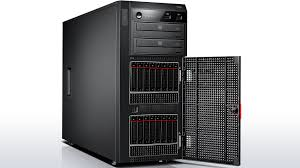
\includegraphics[height=2cm]{hw_tower.jpg} 
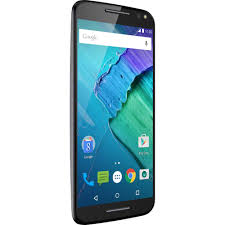
\includegraphics[height=2cm]{hw_smartphone.jpg}
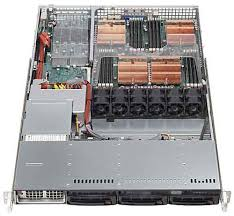
\includegraphics[height=2cm]{server_1u.jpg}
	\begin{itemize}
            \item Is it possible to work without OS?
            \item Why it is necessary?
	    \item What does OS do?
	\end{itemize}
\end{frame}

\begin{frame}{Operation system GNU/Linux components.}
    \begin{columns}
        \column{0.6\textwidth}
    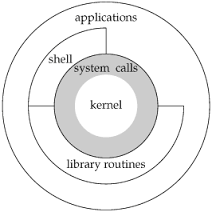
\includegraphics[scale=1]{unix_arch_highlevel}
        \column{0.4\textwidth}
	\begin{itemize}
		\item Kernel (Linux)
		\item Libraries (glibc)
                \item Compiler (GCC) 
		\item System utilities and applications (Userspace)
	\end{itemize}
    \end{columns}
\end{frame}
}
\mode<all>{\begin{frame}[fragile]{Задачи ядра Linux}
    \begin{columns}
    \column{0.6\textwidth}
        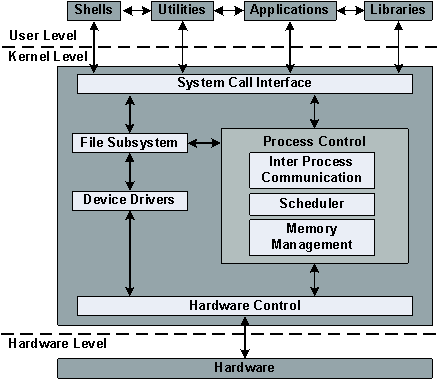
\includegraphics[scale=0.63]{unix_arch_details}
    \column{0.4\textwidth}
	\begin{itemize}
		\item Драйвера устройств
		\item Инициализация системы
		\item Управление
                    \begin{itemize}
                        \item процессами и потоками
                        \item памятью
                        \item файлами
                    \end{itemize}
		\item IPC (Inter Process Communication)
		\item Разграничение доступа
	\end{itemize}
    \end{columns}
\end{frame}
}
% Задачи ядра Linux
%\mode<all>{\begin{frame}{Задачи ядра Linux}
	\begin{itemize}
		\item Инициализация системы
		\item Управление процессами и потоками
		\item Управление памятью
		\item Управление файлами
		\item IPC (Inter Process Communication)
		\item Разграничение доступа
		\item Сетевые возможности
		\item Интерфейс доступа к возможностям ядра
	\end{itemize}
	%Выполнить команду dmesg и найти строки инициализации памяти, CPU, дисковой подсистемы, CPU.
\end{frame}
}
\section{Виртуализация.}
\mode<all>{\begin{frame}
\frametitle{A non-virtualized computer}
    \center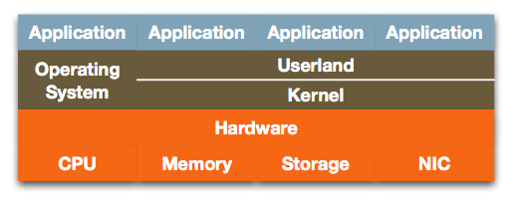
\includegraphics[width=8cm]{hardware.png}
\end{frame}
}
\mode<all>{\begin{frame}
\frametitle{Running one application per server}
\begin{itemize}
    \item \alert{Application-specific requirements:} run only on specific versions of an OS with a specific patch level. 
    \item \alert{Application conflict:}  incompatible with each other.
    \item \alert{Resource contention:} A heavily-used application cannot crowd out other applications
    \item \alert{Resilience:} crashes won't bring down other applications.
    \item \alert{Maintenance:} upgrade and reboot one system without affecting others.
\end{itemize}
The one-app-per-server model worked well in the 1980s and 1990s.  Powerful servers  utilization was only 8-15\% 
\end{frame}
}
\mode<all>{\begin{frame}
\frametitle{Hosted virtualization}
    \center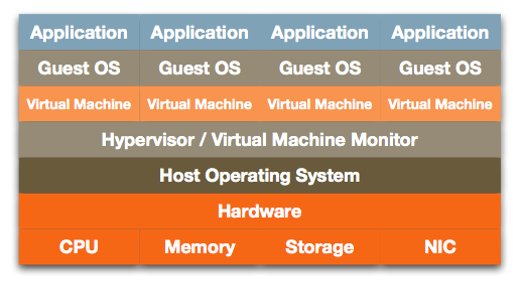
\includegraphics[width=9cm]{vm_hosted.png}
\end{frame}
}
\mode<all>{\begin{frame}
\frametitle{Bare-Metal Hardware virtualization} 
    Proxmox, VMware vSphere (ESXi)
    \center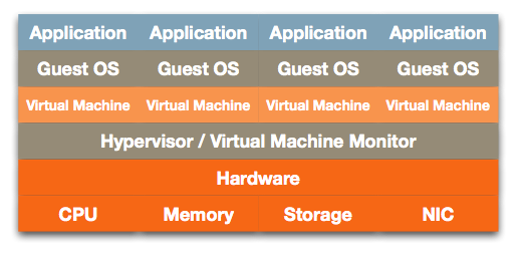
\includegraphics[width=9cm]{bare_metal_virtualization.png}
\end{frame}
}
\mode<all>{\begin{frame}
\frametitle{Paravirtualization}
    \center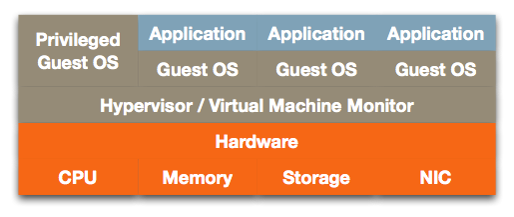
\includegraphics[width=9cm]{hypervisor.png}
\end{frame}
}
\mode<all>{\begin{frame}
\frametitle{Oracle VirtualBox. VM creation steps}
\begin{itemize}
    \item 
Create Virtual Machine
    \item 
Specify memory size
    \item 
Specify disk size, type, dynamic vs fixed size
\end{itemize}
\end{frame}
}
\mode<all>{\begin{frame}
\frametitle{Virtualbox NAT Networking}
    \center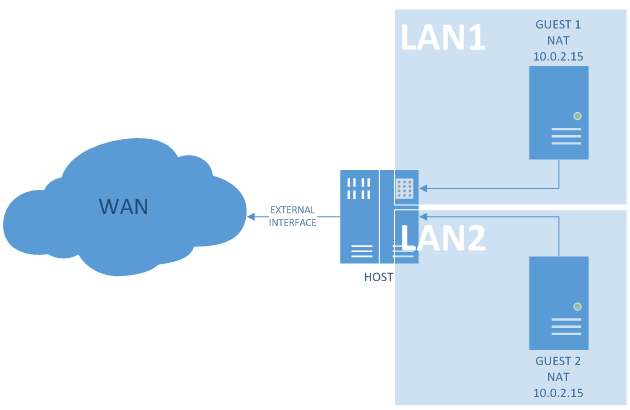
\includegraphics[width=9cm]{vm_nat01.png}
\end{frame}
}
\mode<all>{\begin{frame}
\frametitle{Virtualbox Network Host Only}
	\begin{columns}
	\column{0.5\textwidth}
        \begin{itemize}
            \item Встроенный DHCP сервер
            \item Доступ из хост системы
            \item Доступ к соседним виртуальным машинам
        \end{itemize}
	\column{0.5\textwidth}
    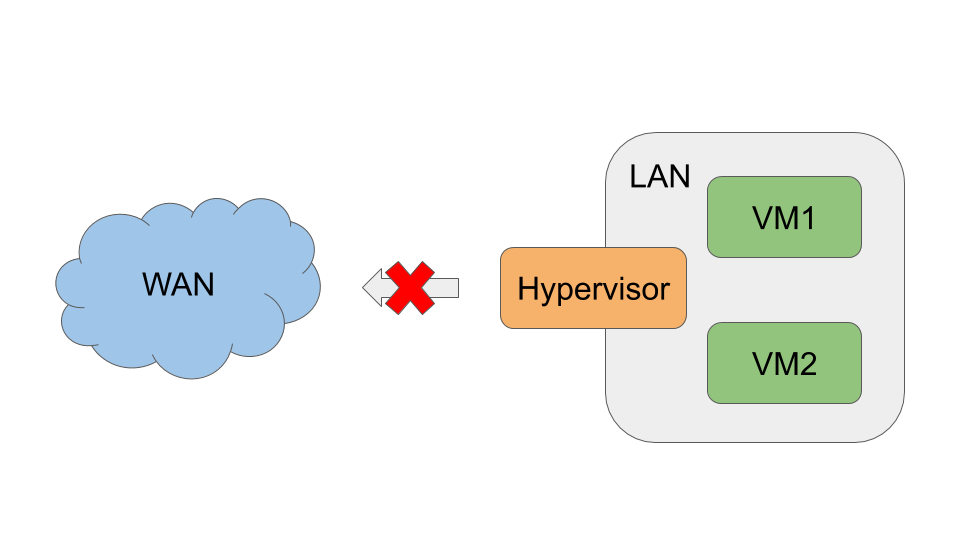
\includegraphics[height=0.4\textheight]{../../slides/vbox/Virtualbox network HostOnly.png}
	\end{columns}
\end{frame}}
\mode<all>{\begin{frame}
\frametitle{Virtualbox Network Bridge}
	\begin{columns}
	\column{0.5\textwidth}
        \begin{itemize}
            \item Нужен внешний DHCP сервер
            \item Доступ в Internet
            \item Доступ из хост системы
            \item Доступ к соседним виртуальным машинам
        \end{itemize}
	\column{0.5\textwidth}
    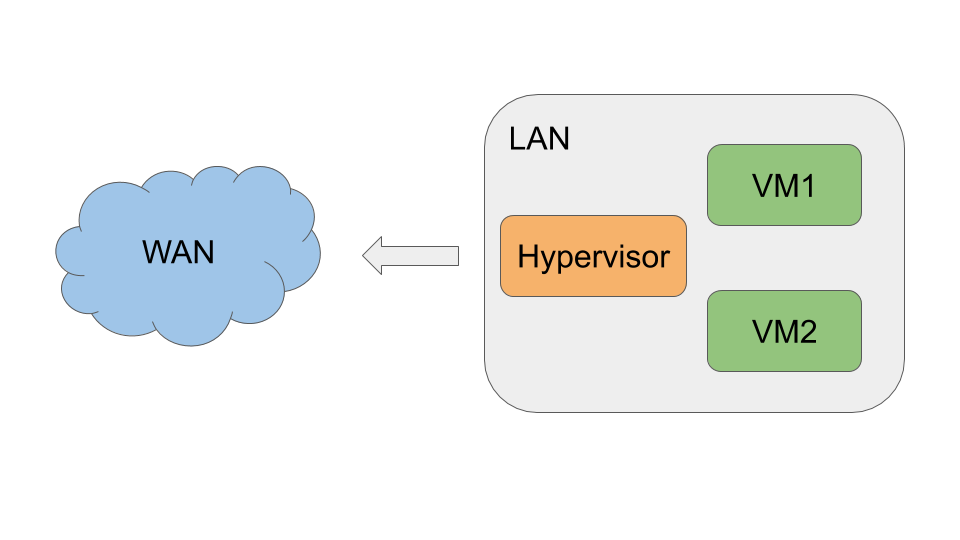
\includegraphics[height=0.4\textheight]{../../slides/vbox/Virtualbox network Bridge.png}
	\end{columns}
\end{frame}
}
\mode<all>{\begin{frame}
\frametitle{Virtualbox Internal Network}
	\begin{columns}
	\column{0.5\textwidth}
        \begin{itemize}
            \item Доступ к соседним виртуальным машинам
        \end{itemize}
	\column{0.5\textwidth}
    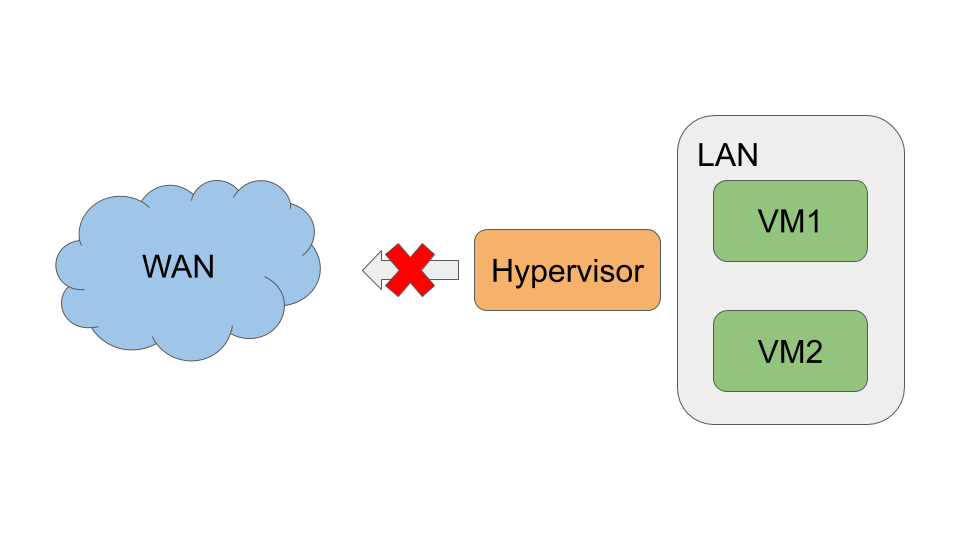
\includegraphics[height=0.4\textheight]{../../slides/vbox/Virtualbox network Internal.png}
	\end{columns}
\end{frame}}
\mode<all>{\begin{frame}
\frametitle{Typing special characters}

Special key combinations with the \alert{Host key} (normally the 
\alert{right Control key}) 
\begin{itemize}
\item \alert{Host key} to return back to host system from virtual machine
\item \alert{Host key + Del} to send Ctrl+Alt+Del (to reboot the guest);
\item \alert{Host key + F1} (or other function keys) to simulate Ctrl+Alt+F1
\end{itemize}
\end{frame}
}

\section{Дистрибутивы ОС Linux}
% TODO ISO example
% TODO setup methods
\mode<all>{\begin{frame}{Задачи дистрибутива}
	\begin{itemize}
		\item Предоставление комплекта ПО. 
		\item Средства установки и настройки
		\item Средства обновления
	\end{itemize}
        Обычно дистрибутив состоит из ПО с открытым исходным кодом, который можно скачать из сети, собрать и установить самостоятельно.  Задча трудозатратная по времени. \\
Разрабочики дистрибутивов уже выполнили ее, поэтому пользователи используют готовый дистрибутив.
\end{frame}
}
\mode<all>{\begin{frame}{Разнообразие Linux дистрибутивов и проблема выбора.}
    Угадайка. Сколько по вашему мнению существует активных дистрибутивов? 
    \pause
    \alert{257} - по версии distrowatch.com. \break 
    Что и как выбрать? \pause 
    \break
Все зависит от нас самих.  \break
    Выбор дистрибутива определяется:
	\begin{itemize}
            \item нашим железом;
            \item умением и опытом работы;
            \item нашими задачами;
	\end{itemize}
\end{frame}

\begin{frame}{Выбор дистрибутивов для обучения}
    Ubuntu (Debian) \\
    CentOS (Redhat)
	\begin{itemize}
            \item работают на amd64 (старые версии x86), в виртуальных машинах;
            \item распрoстранены на проектах заказчиков;
            \item идеально подходят для обучения: дружественны к пользователю,
            просты в установке и настройке; 
            \item у меня есть опыт работы с обоими дистрибутивами; 
	\end{itemize}
\end{frame}
}
\mode<all>{\begin{frame}{Примеры популярных Linux дистрибутивов.}
	\begin{itemize}
		\begin{columns}
		\column{0.3\textwidth}
			\item RedHat
			\item Fedora Core
			\item CentOS
			\item Scientific Linux
			\item Oracle Unbreakable Linux
		\column{0.3\textwidth}
			\item Slackware 
			\item Gentoo
			\item Arch
			\item OpenSUSE
			\item ALT Linux 
		\column{0.3\textwidth}
			\item Debian
			\item Ubuntu
			\item Mint
			\item Knoppix
			\item BackTrack
		\end{columns}
	\end{itemize}
    \begin{itemize}
        \item По назначению серверный или десктопный; 
        \item По скорости обновления: стабильный или обновляющийся; 
    \end{itemize}
\end{frame}
}
\mode<all>{\begin{frame}{Различия между дистрибутивами.}
	\begin{itemize}
		\begin{columns}
		\column{0.4\textwidth}
			\item Система управления пакетами (может отсутствовать)
			\item Формат распространения ПО
			\item Система сборки ПО
			\item Пути к файлам
            \item Документация
		\column{0.4\textwidth}
			\item Инсталлятор
			\item Первичные настройки
			\item Средства управления
			\item Набор ПО
		\end{columns}
	\end{itemize}
\end{frame}

\begin{frame}{Сходство между дистрибутивами.}
    \begin{itemize}
        \item Ядро Linux представляет собой Unix-like OS. 
        \item Linux API совместим со стандартом POSIX, Single UNIX Specification (SUS). 
        \item Стандартный набор команд и аргументов доступный из интерактивной оболочки. 
        \item Расположение и название файлов
    \end{itemize}
\end{frame}
}
\mode<all>{\begin{frame}{Installation methods}
	\begin{itemize}
            \item Install from existing Linux 
            \item Network installation 
            \item Use preinstalled virtual machine image (cloud)
            \item Write the image on flash media or optical disc
	\end{itemize}
\end{frame}
}
% activity ISO list what info can you get from ISO names?
\mode<all>{\begin{frame}{Установка с ISO образа}
    Что можно сказать о дистрибутиве по имени образа?
	\begin{enumerate}
            \item debian-8.5.0-amd64-netinst.iso
            \item CentOS-7-x86\_64-DVD.iso
            \item debian-8.5.0-powerpc-DVD-1.iso
            \item openSUSE-Leap-42.1-DVD-x86\_64.iso
            \item archlinux-2016.08.01-dual.iso
	\end{enumerate}
\end{frame}
}
\end{document}
\bye
